\documentclass[10pt]{beamer}
\usetheme[
%%% option passed to the outer theme
%    progressstyle=fixedCircCnt,   % fixedCircCnt, movingCircCnt (moving is deault)
  ]{Feather}
  
% If you want to change the colors of the various elements in the theme, edit and uncomment the following lines

% Change the bar colors:
%\setbeamercolor{Feather}{fg=red!20,bg=red}

% Change the color of the structural elements:
%\setbeamercolor{structure}{fg=red}

% Change the frame title text color:
%\setbeamercolor{frametitle}{fg=blue}

% Change the normal text color background:
%\setbeamercolor{normal text}{fg=black,bg=gray!10}

%-------------------------------------------------------
% INCLUDE PACKAGES
%-------------------------------------------------------

% General
\usepackage[utf8]{inputenc}
\usepackage[portuguese]{babel}
\usepackage[T1]{fontenc}
\usepackage{helvet}

% Code syntax highlight
\usepackage{setspace}
\usepackage{color}
\usepackage{listings}

% Specify table cell length
\usepackage{array}

% Hyperlink reference
\usepackage{hyperref}

%-------------------------------------------------------
% DEFFINING AND REDEFINING COMMANDS
%-------------------------------------------------------

% colored hyperlinks
\newcommand{\chref}[2]{
  \href{#1}{{\usebeamercolor[bg]{Feather}#2}}
}

%-------------------------------------------------------
% Configure syntax highlight
%-------------------------------------------------------
\lstset{
  backgroundcolor=\color{white},
  breaklines=true,
  commentstyle=\color{green},
  extendedchars=true,
  frame=single,
  keepspaces=true,
  keywordstyle=\color{blue},
  language=Ruby,
  numbers=left,
  numbersep=10pt,
  numberstyle=\small\color{gray},
  rulecolor=\color{black},
  stringstyle=\color{blue},
  tabsize=2
}
%-------------------------------------------------------
% INFORMATION IN THE TITLE PAGE
%-------------------------------------------------------

% [] is optional - is placed on the bottom of the sidebar on every slide
% is placed on the title page
\title[] { 
\textbf{Kuniri Project}
}

\subtitle[An overview] {
}

\author[kuniri presentation] {
Rodrigo Siqueira Jordão
}

\date{\today}

%-------------------------------------------------------
% THE BODY OF THE PRESENTATION
%-------------------------------------------------------

\begin{document}

%-------------------------------------------------------
% THE TITLEPAGE
%-------------------------------------------------------

{\1% % this is the name of the PDF file for the background
% the plain option removes the header from the title page, noframenumbering removes the numbering of this frame only
\begin{frame}[plain,noframenumbering] 
  \titlepage % call the title page information from above
\end{frame}
}

\begin{frame}{Summary}{}
  \tableofcontents
\end{frame}

%=======================================================
\section{Introduction}
%=======================================================
\begin{frame}{Introduction}{Overview}
  \begin{figure}[ht]
    \centering
    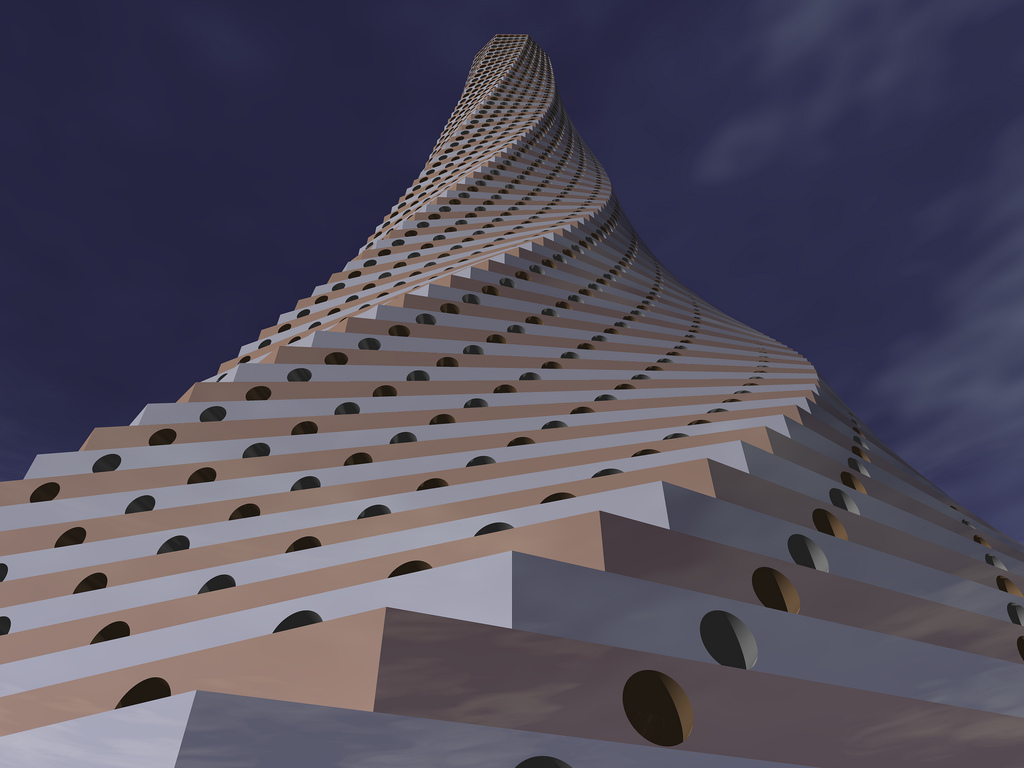
\includegraphics[width=0.85\textwidth, keepaspectratio=true]{images/introduction.jpg}
  \end{figure}
\end{frame}

\begin{frame}{Introduction}{Overview}
  \begin{figure}[overview]
    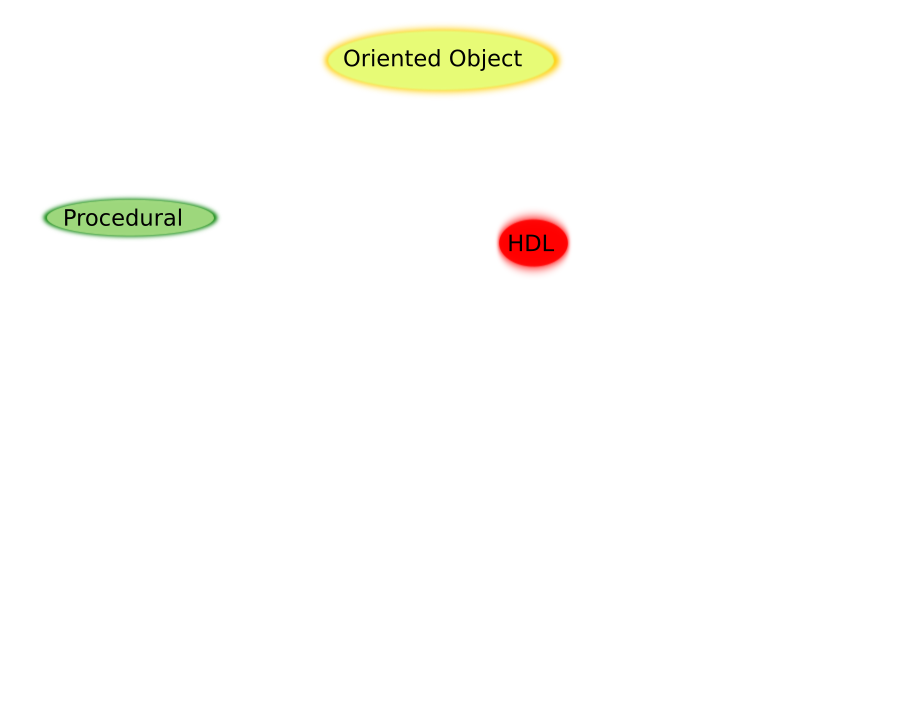
\includegraphics[width=0.7\textwidth]{images/paradigms.png}
  \end{figure}
\end{frame}

\begin{frame}{Introduction}{Overview}
  \begin{figure}[overview]
    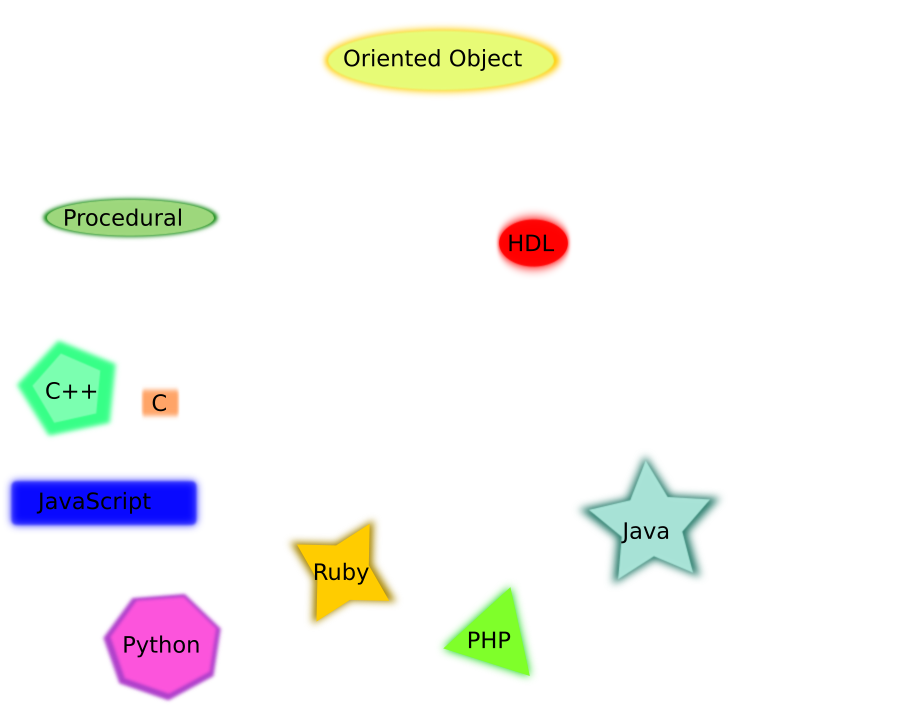
\includegraphics[width=0.7\textwidth]{images/paradigmAndLanguages.png}
  \end{figure}
\end{frame}

\begin{frame}{Introduction}{Overview}
  \begin{figure}[overview]
    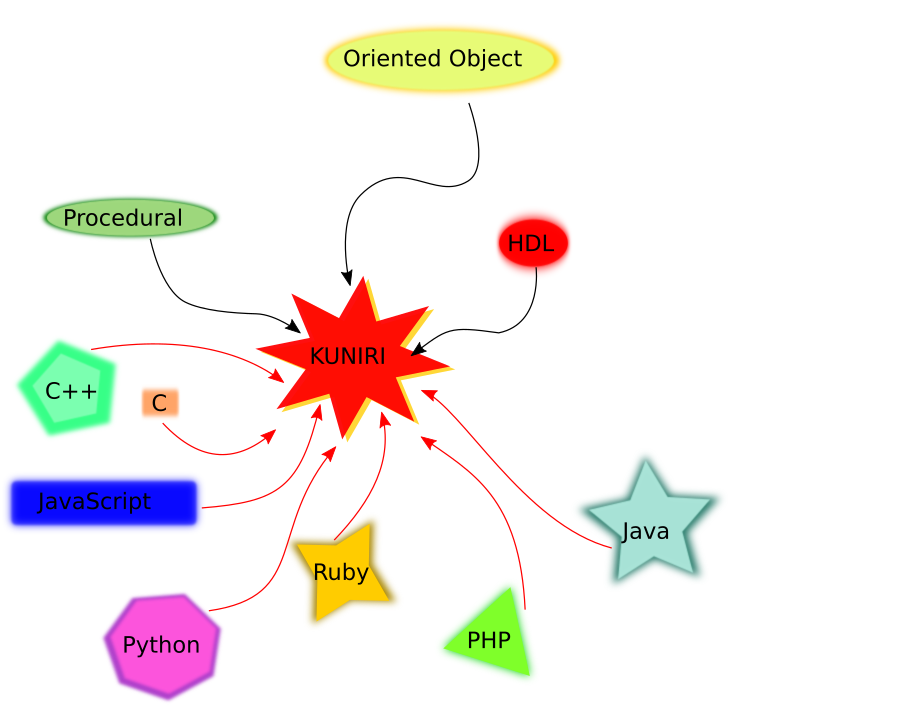
\includegraphics[width=0.7\textwidth]{images/paradigmAndLanguagesAndKuniri.png}
  \end{figure}
\end{frame}

\begin{frame}{Introduction}{Overview}
  \begin{figure}[overview]
    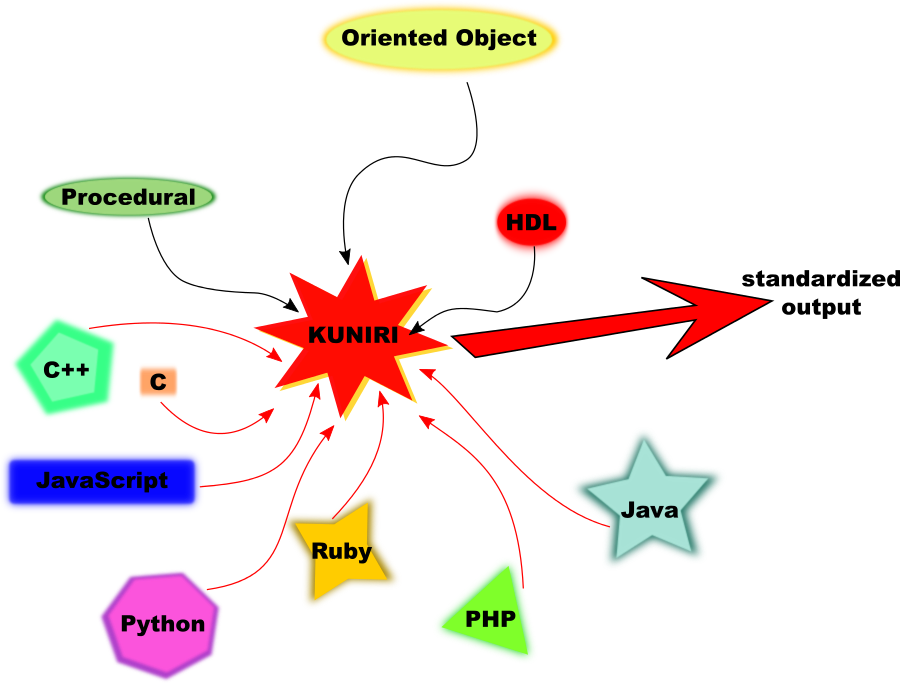
\includegraphics[width=0.7\textwidth]{images/overview.png}
  \end{figure}
\end{frame}

%-------------------------------------------------------
\begin{frame}{Introduction}{History}
\end{frame}

%-------------------------------------------------------
\begin{frame}{Introduction}{About our logo}
  \begin{figure}[overview]
    
\includegraphics[width=0.3\textwidth]{images/kuniri.png}
  \end{figure}
\end{frame}

%-------------------------------------------------------
\begin{frame}{Introduction}{About our organization}

\end{frame}

%=======================================================
\section{Kuniri Architecture}
%=======================================================
\begin{frame}{Architecture}{Overview}
\end{frame}

%-------------------------------------------------------
\begin{frame}{Architecture}{Container Data}
\end{frame}

%-------------------------------------------------------
\begin{frame}{Architecture}{Abstract Container}
\end{frame}

%-------------------------------------------------------
\begin{frame}{Architecture}{State Machine}
\end{frame}
%-------------------------------------------------------

%=======================================================
\section{Law of Demeter inside Kuniri}
%=======================================================
\begin{frame}{Law of Demeter}{Overview}
\end{frame}

%-------------------------------------------------------
\begin{frame}[fragile]{Law of Demeter}{Real code}
\small
\begin{lstlisting}
...
def execute(pElementFile, pLine)
  attributeElement = @language.attributeHandler.get_attribute(pLine)
  if attributeElement
    lastIndex = pElementFile.classes.length - 1
    attributeElement.each do |attribute|
      attribute.comments = @language.string_comment_to_transfer
    end
    @language.string_comment_to_transfer = ''
    pElementFile.classes[lastIndex].add_attribute(attributeElement)
  end
...
\end{lstlisting}
\end{frame}

\begin{frame}[fragile]{Law of Demeter}{Apply LoD}
\small
\begin{lstlisting}
...
class FileElementData < Languages::BasicData
...
 def add_attribute_to_last_class(pAttributeElement)
  classes.last.add_attribute(pAttributeElement)
 end
...
end
\end{lstlisting}
\end{frame}

%-------------------------------------------------------
\begin{frame}{Law of Demeter}{Singleton and Law of Demeter}
\end{frame}

\begin{frame}{Law of Demeter}{Fluid interfaces}
\end{frame}

%=======================================================
\section{Running kuniri and output}
%=======================================================
\begin{frame}{Running}{Example}
\end{frame}

%=======================================================
\section{Conclusions}
%=======================================================
\begin{frame}{Conclusion}{}
\end{frame}

{\1
\begin{frame}[plain,noframenumbering]
  \finalpage{Thanks!}
\end{frame}}

\end{document}
